\documentclass[hyperref={pdfpagelabels=false}]{beamer} 

\usepackage{sfocs-poster}

\usebackgroundtemplate{%
	\begin{tikzpicture}[remember picture,overlay] 
		% set a background color
		\fill[top color=black!70, bottom color=black] (current page.north west) rectangle (current page.south east); 
		% image as background
%		\node[inner sep=0pt,outer sep=0pt] at (current page.center) {\includegraphics[height=\paperheight,width=\paperwidth,keepaspectratio]{img/background3}};
	\end{tikzpicture}
}

% \newfontfamily\comic{Comic Sans MS}

% an octagonal box
\newtcolorbox{octobox}[1][]{nobeforeafter, size=minimal,auto outer arc,octogon arc, halign=center,valign=center, square,arc is angular,#1}


% draw a grid: helpful to ensure elements are perfectly aligned
%\beamertemplategridbackground[1cm]

\begin{document}

\begin{frame}

%
% poster content arranged in boxes
%

\begin{textblock}{65}(15,2)
	\begin{blankbox}[fontupper=\comic\fontsize{85}{45}\selectfont,colupper=white!75,halign=center]
		Big Data Analysis on Million Song Dataset \\
		\vspace{0.5 cm}
		\huge Yiding Chang, Kexuan Huang, Yifan Shen, Qinghang Wu
	\end{blankbox}
\end{textblock}

\begin{textblock}{40}(9,12.5)
	\begin{basebox}[title=Introduction,opacitybacktitle=.45,colframe=green!65!black,colbacktitle=green!10, halign title=left]
		To build a successful music platform, this project aims at developing an efficient music recommendation system with Hadoop, Drill, and Spark. Our goals are as follows.
		\vspace{0.15 cm}
		\begin{itemize}
		\item Use Drill to conduct basic analysis on the million song dataset. 
		\item Use parallel Breadth First Search (BFS) to calculate the similarities and differences between artists.
		\end{itemize}
	\vspace{0.15 cm}
	\end{basebox}
\end{textblock}

\begin{textblock}{40}(9,32.5)
	\begin{basebox}[title=Proposed Work Flow,opacitybacktitle=.45,colbacktitle=green!10,colframe=green!65!black, halign title=left]
		In order to efficiently conduct the analysis, we propose to follow the below work flow with three milestones. 
		\vspace{0.3 cm}
		\begin{figure}[H]
		  \center
		  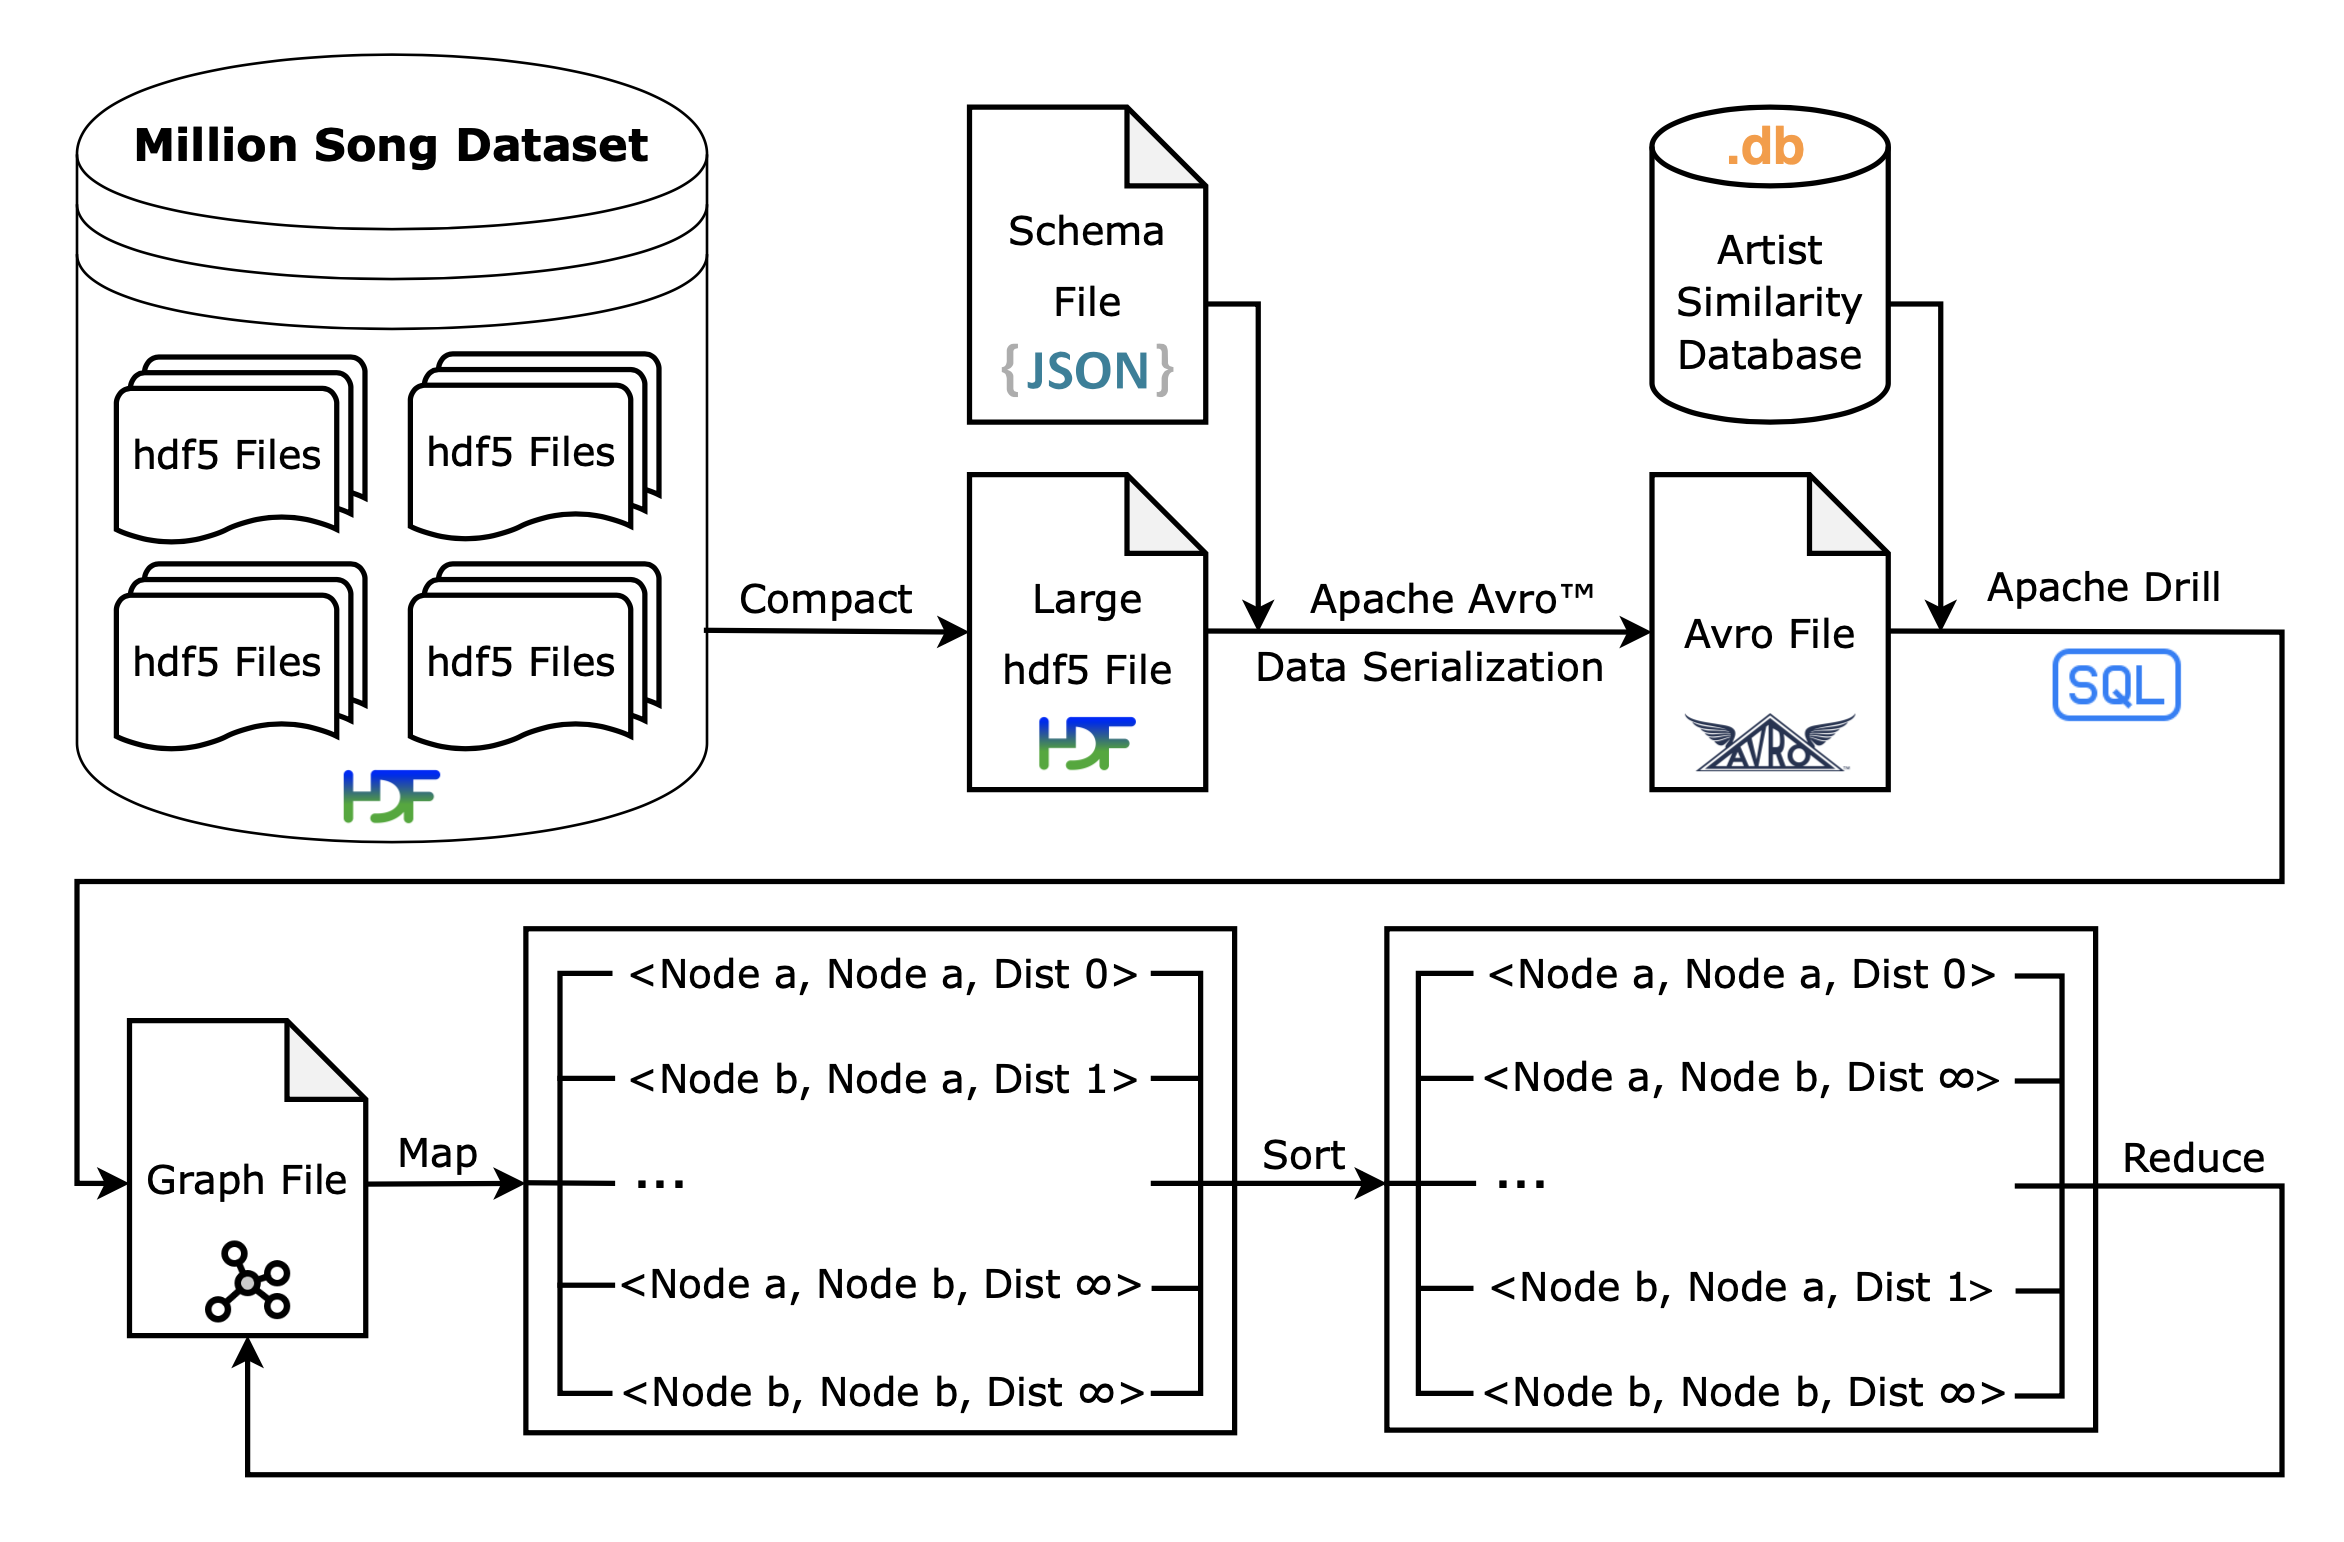
\includegraphics[width=0.9\linewidth]{workflow.PNG}
		  \caption{Work flow of the project}
		\end{figure}
	\vspace{0.2 cm}
	\end{basebox}
\end{textblock}

% \begin{textblock}{40}(9,80)
% 	\begin{basebox}[title=Data Preprocessing, opacitybacktitle=.45,colbacktitle=green!10, halign title=left]
% 		xxx
% 		\vspace{5 cm}
% 	\end{basebox}
% \end{textblock}


\begin{textblock}{40}(9,78)
	\begin{basebox}[title=Basic Data Analysis,opacitybacktitle=.45,colframe=green!65!black,colbacktitle=green!10, halign title=left]
		To test on the compacted dataset, we use drill to query one of the sub dataset and retrieve the following information: 
		\vspace{0.3 cm}
		\begin{itemize}
		\item The oldest song is 96 years old, while the youngest is 12 years old.
		\item Hottest song that is the shortest and shows highest energy with lowest tempo is `Immigrant Song (Album Version)'. 
		\item `Greatest Hits' has the most tracks, which is, 21. 
		\item Name of the band who recorded the longest song is `UFO'. 
		\end{itemize}
	\end{basebox}
\end{textblock}

% \begin{textblock}{40}(51,12.5)
% 	\begin{basebox}[title=Parallel BFS Algorithm,opacitybacktitle=.45,colbacktitle=green!10, halign title=left]
% 		To parallelize BFS, we propose the following algorithm,  
% 		\vspace{31.5 cm}
% 	\end{basebox}
% \end{textblock}

\tcbset{frogbox/.style={enhanced,colbacktitle=green!10,colframe=green!65!black,
		enlarge top by=5.5mm,
		overlay={\foreach \x in {-5.5cm,-8cm} {
				\begin{scope}[shift={([xshift=\x]frame.north east)}]
				\path[draw=green!65!black,fill=green!10,line width=2mm] (0,0) arc (0:180:1cm);
				\path[fill=black] (-0.2,0) arc (0:180:3mm);
\end{scope}}}}}

\begin{textblock}{40}(51,11.7)
	\begin{basebox}[frogbox,title=Parallel BFS Algorithm, opacitybacktitle=.45, halign title=left]
 		For BFS with MapReduce, we used the following algorithm and implemented it in Python,   
 		\begin{enumerate}
 			\item Initialize graph file with target artists in the format of `Node,  Distance, Neighbors'
 			\item Mapper: Generate neighbors, Node, Distance $+1$ if not itself
 			\item Reducer: Merge the same neighbor, keep distance minimum
 		\end{enumerate}
 		\begin{figure}[H]
 		\minipage{0.32\textwidth}
		  \center
		  \includegraphics[width=0.98\linewidth]{step1.PNG}
		  \caption{Initialize Graph File}
		\endminipage\hfill
		\minipage{0.32\textwidth}
		  \center
		  \includegraphics[width=0.98\linewidth]{step2.PNG}
		  \caption{Graph after 1 MapReduce Iteration}
		\endminipage\hfill
		\minipage{0.32\textwidth}
		  \center
		  \includegraphics[width=0.98\linewidth]{step3.PNG}
		  \caption{Graph after 2 MapReduce Iterations}
		\endminipage\hfill
		\end{figure}
 		\vspace{0.1 cm}
 		For BFS with Spark, we implemented it using Python with `PySpark' with the following steps: 
 		\begin{enumerate}
 			\item Convert data into RDD map
 			\item Using Spark `sortByKey()' to sort RDD aggregated by node index and then combining the neighbours
 			\item Using Spark `reduce()' to pick the minimum distance of different neighbours towards the central node
 		\end{enumerate}
		\vspace{0.1 cm}
 		The data size we used is around 200GB. The server we used is SJTU cluster with three machines with CPU of Dual-core Intel Xeon Processor (Skylake, IBRS) and memory of 4GB.
	\end{basebox}
\end{textblock}


\begin{textblock}{40}(51,75.5)
	\begin{basebox}[title=Conclusion, opacitybacktitle=.45,colbacktitle=green!10, colframe=green!65!black, halign title=left]
 With big data technology, we have successfully implemented parallel BFS algorithms in both MapReduce and Spark to determine the similarities and differences between the artists. To summarize, 
 \begin{itemize}
\item Conducting basic queries on the dataset can provide lots of insights about the music industry.
\item When running on the whole 200 GB dataset, on average, MapReduce finishes the task around 250s, while Spark finishes the task around 45s. Therefore, we conclude Spark is 5.5 times faster than MapReduce, so it would be a better option for the music platform. 
\end{itemize}
	\end{basebox}
\end{textblock}

%
% extra content (logos, dev comments, acknowledgements, etc.)
%

\begin{textblock}{22.75}[1,0](110,2.5)
	\logos[light]
\end{textblock}

\end{frame}

\end{document}